%% One Trace Is Not Enough: Hyperproperty Grading for Agent-Authored Control Systems
%% Artifact: https://github.com/pandeyaby/DIPTYCH (MIT). Build: make paper.
%% Reproduce Table IV: python -m diptych.adequacy · Table V: python -m diptych.pilot.study
%% Adapter pins (checked by diptych-pins against adapters/PINS.md): ZeroDay@fb5b39da · AOMB@667e475

\documentclass[conference]{IEEEtran}
\IEEEoverridecommandlockouts

\usepackage{amsmath}
\usepackage{amssymb}
\usepackage{amsthm}
\usepackage{booktabs}
\usepackage{graphicx}
\usepackage{url}
\usepackage{balance}

% Compile from paper/: figures live under docs/images/
\graphicspath{{../docs/images/}{docs/images/}}

\newtheorem{proposition}{Proposition}
\newtheorem{definition}{Definition}
\newtheorem{corollary}{Corollary}

\newcommand{\sys}{\textsc{Diptych}}
\newcommand{\Tr}{\mathrm{Tr}}
\newcommand{\exec}{\mathrm{exec}}

\begin{document}
	
	\title{One Trace Is Not Enough: Hyperproperty Grading\\for Agent-Authored Control Systems}
	
	% --- Author block switch (see paper/ANON.md) ---
	% Default: camera-ready / single-blind (named authors).
	% Double-blind: comment the named block and uncomment the anonymous block.
	\author{
		\IEEEauthorblockN{Abhinav Pandey}
		\IEEEauthorblockA{Independent Researcher\\
			pandey.aby@gmail.com}
		\and
		\IEEEauthorblockN{Abhishek Pandey}
		\IEEEauthorblockA{Meta\\
			pandeyabhi1987@gmail.com}
	}
	% \author{
	% 	\IEEEauthorblockN{Anonymous Author(s)}
	% 	\IEEEauthorblockA{Paper under double-blind review\\
	% 		Anonymous Institution(s)\\
	% 		Correspondence via conference submission system only}
	% }
	
	\maketitle
	
	\begin{abstract}
		Agentic coding benchmarks grade a candidate artifact from a single
		execution trace. We show that this model cannot express many requirements
		on agent-authored systems. Properties such as calibrated conservatism
		under volatility, anti-windup, reproducibility across restarts, and
		telemetry schema stability are \emph{hyperproperties}: predicates over
		sets of traces, which in general no single execution can falsify.
		
		We make three contributions. First, a property taxonomy for agentic
		evaluation and an audit of a public controller specification, the
		IETF's criteria for evaluating congestion control algorithms (RFC~9743):
		eight of its eighteen behavioral criteria are defined by a contrast
		between two executions. We prove the obstruction:
		two stateful deterministic artifacts can produce the identical trace yet
		respond with opposite asymmetry, so no single-trace estimate identifies it.
		
		Second, \sys{}, a grading harness that renders every hyperproperty
		judgment on a coupled pair: eight perturbation operators, a coupling
		discipline for closed-loop pairs, and a probe-tree strategy that
		amortizes a shared prefix.
		
		Third, an evaluation. A mutation sweep over every conforming probe
		(1{,}030 mutants) exposed three classes of defect in our own graders.
		In a pilot with 80 controllers written by Claude and OpenAI models on
		two tasks, the answer depends on where the reference comes from. On a
		concurrency task whose requirements compare an artifact with itself at
		a fixed state, 28 of the 34 controllers that pass every single-trace
		check violate a requirement stated in plain words. On a congestion
		task built from RFC~9743, a single run catches every case of harm to a
		standard flow, because the reference outcome is a known constant, and
		pairing adds only the history-dependent violations. One trace is not
		enough exactly when the reference depends on the artifact's own state.
	\end{abstract}
	
	\begin{IEEEkeywords}
		agentic benchmarks, hyperproperties, metamorphic testing, evaluation
		methodology, autonomic control, LLM code generation
	\end{IEEEkeywords}
	
	\section{Introduction}
	
	The dominant evaluation model for agent-authored software is trace scoring.
	A benchmark supplies an input, the artifact runs, and a grader inspects what
	came out: a test suite verdict, a task completion flag, a reward from a
	simulated environment, or a language-model judgment over a recorded
	trajectory. The unit of judgment is one execution.
	
	This model is adequate when the requirement is itself a property of one
	execution. ``The function returns the correct value'' and ``the agent
	eventually books the flight'' are both decided by watching a single run.
	Much of what we want from autonomous systems is not of this form. Consider
	four requirements on an adaptive concurrency controller, from the task we
	release with this paper (Section~\ref{sec:pilot}):
	
	\begin{itemize}
		\item \textbf{Asymmetric response.} The controller's downward correction to
		a deviation from setpoint must strictly exceed twice its upward correction
		to a deviation of equal magnitude and opposite sign.
		\item \textbf{Volatility suppression.} Given two workloads with equal mean
		and different variance, the controller must converge to a strictly more
		conservative limit on the higher-variance workload.
		\item \textbf{Anti-windup.} After sustained saturation at a ceiling, the
		first response to a latency excursion must be bounded by the immediately
		observed error and not by how long the controller was saturated.
		\item \textbf{Determinism.} The same configuration and observation sequence
		must yield a bit-identical decision sequence across fresh interpreter
		processes.
	\end{itemize}
	
	None of these can be falsified by examining one trace. Each is a statement
	relating two or more executions. Determinism is the textbook case: it is
	the observational-determinism hyperproperty from the information-flow
	literature, and it is well understood there that it is not a trace property
	\cite{clarkson2010,zdancewic2003}. Our claim is that the other three are
	formally the same kind of object and that this class captures the
	judgment and calibration we most want to measure in agent-authored
	systems. Such requirements are not peculiar to our task: the IETF's
	guidance for assessing congestion controllers asks whether a new
	algorithm causes more harm to competing flows than a standard one
	would \cite{rfc9743}, a comparison between two runs.
	
	The practical consequence is a silent failure mode in benchmark design. A
	specification author writes an invariant in single-trace prose. A harness
	author implements a single-trace check that appears to match the prose. The
	check passes on artifacts that violate the intent, because the discriminating
	evidence never appears in one run. The benchmark reports a score, the score
	is wrong, and nothing in the pipeline signals the gap.
	
	\subsection{Contributions}
	
	\begin{enumerate}
		\item \textbf{A property taxonomy for agentic evaluation} (Section
		\ref{sec:taxonomy}). We classify grading targets into trace safety,
		quantitative trace properties, $k$-safety hyperproperties, quantitative
		hyperproperties, and resource properties, and we state for each what
		evidence is required to falsify it.
		
		\item \textbf{An audit of a public specification} (Section \ref{sec:audit}).
		We classify the eighteen behavioral evaluation criteria of RFC~9743, the
		IETF's Best Current Practice for assessing congestion control
		algorithms. Eight are defined by a counterfactual contrast---harm,
		impact, or robustness relative to a reference run---and the document
		prescribes neither thresholds nor how to construct the comparison.
		
		\item \textbf{A state-confounding obstruction} (Proposition
		\ref{prop:confound}). For a deterministic stateful transducer on a
		non-repeating observation stream, no single trace supplies both arms of the
		counterfactual contrast that an asymmetry invariant requires: two
		artifacts can produce the identical trace yet have contrasts of opposite
		sign. Under a black-box contract, paired execution from a shared state
		is the construction that identifies the quantity.
		
		\item \textbf{\sys{}, a paired-trace grading harness} (Sections
		\ref{sec:harness} and \ref{sec:operators}). Eight perturbation operators, a
		coupling discipline for closed-loop simulators based on common random
		numbers, a validity check that detects when a pair has drifted out of
		comparability, and a probe-tree execution strategy with an amortized cost
		model (Proposition \ref{prop:prefix}).
		
		\item \textbf{An evaluation} (Section \ref{sec:protocol}). Control
		twins, a power-on-axis gate, and an exhaustive mutation sweep that found
		and fixed real grader defects; and a pilot on 80 model-written
		controllers for two tasks, with executable controls, that locates
		where single-trace grading fails and where it suffices.
	\end{enumerate}

	We are explicit about scope. The pilot is small (80 controllers, two
	tasks; we wrote one task's requirements and the other's thresholds) and
	shows where paired grading changes verdicts, not how models compare.
	
	\section{Motivating Example}
	\label{sec:motivating}
	
	We ground the paper in a concrete task, the first of two used in our
	pilot (Section~\ref{sec:pilot}); its requirements shape the harness
	operators.
	
	\subsection{The running task}
	
	A model or agent writes an adaptive concurrency controller: a constructor,
	\texttt{tick} (observation$\to$decision), and snapshot/restore. Each tick
	it observes latency, a latency setpoint, and offered and admitted load,
	and returns a concurrency limit plus telemetry. The limit determines how
	much load a simulated service admits, which determines the next latency.
	The task states eight requirements in prose, among them the four above.
	We wrote the task and release it with the paper.
	
	\subsection{Two controllers a trace grader cannot separate}
	\label{sec:twoorch}
	
	Consider two candidate artifacts. Both maintain an exponentially weighted
	estimate of latency and adjust a concurrency limit toward a
	setpoint. $A_{\mathrm{sym}}$ applies gain $g$ to the error in both
	directions. $A_{\mathrm{asym}}$ applies $g_{\uparrow}$ when the observed
	latency is below setpoint and $g_{\downarrow}$ when it is above, with
	$g_{\downarrow} > 2 g_{\uparrow}$ and $g_{\uparrow} + g_{\downarrow} = 2g$.
	Only $A_{\mathrm{asym}}$ satisfies the asymmetric-response invariant.
	
	Asymmetric gain on its own shifts the operating point (noise now drives
	the limit down more than up), but other free parameters---setpoint
	offset, estimator bandwidth, gain magnitude---shift it too. $A_{\mathrm{sym}}$
	can therefore be tuned to match $A_{\mathrm{asym}}$ on every aggregate a
	trace grader scores: mean limit, admitted load, latency attainment. Such a
	grader sees two equally good artifacts.
	
	One might object that a single long trace contains both upward and downward
	deviations, so the ratio could be read off directly. It cannot, and the
	reason is the technical heart of the paper. The response to an upward
	deviation at tick $t$ and to a downward deviation at tick $t'$ are responses
	\emph{from different internal states}. The estimator has moved and the
	saturation history differs. Any ratio
	computed across those two moments mixes the sign effect with state drift.
	Proposition \ref{prop:confound} formalizes this. The only construction that
	identifies the sign effect holds the state fixed, which means branching two
	executions from a common prefix.
	
	\begin{figure}[t]
		\centering
		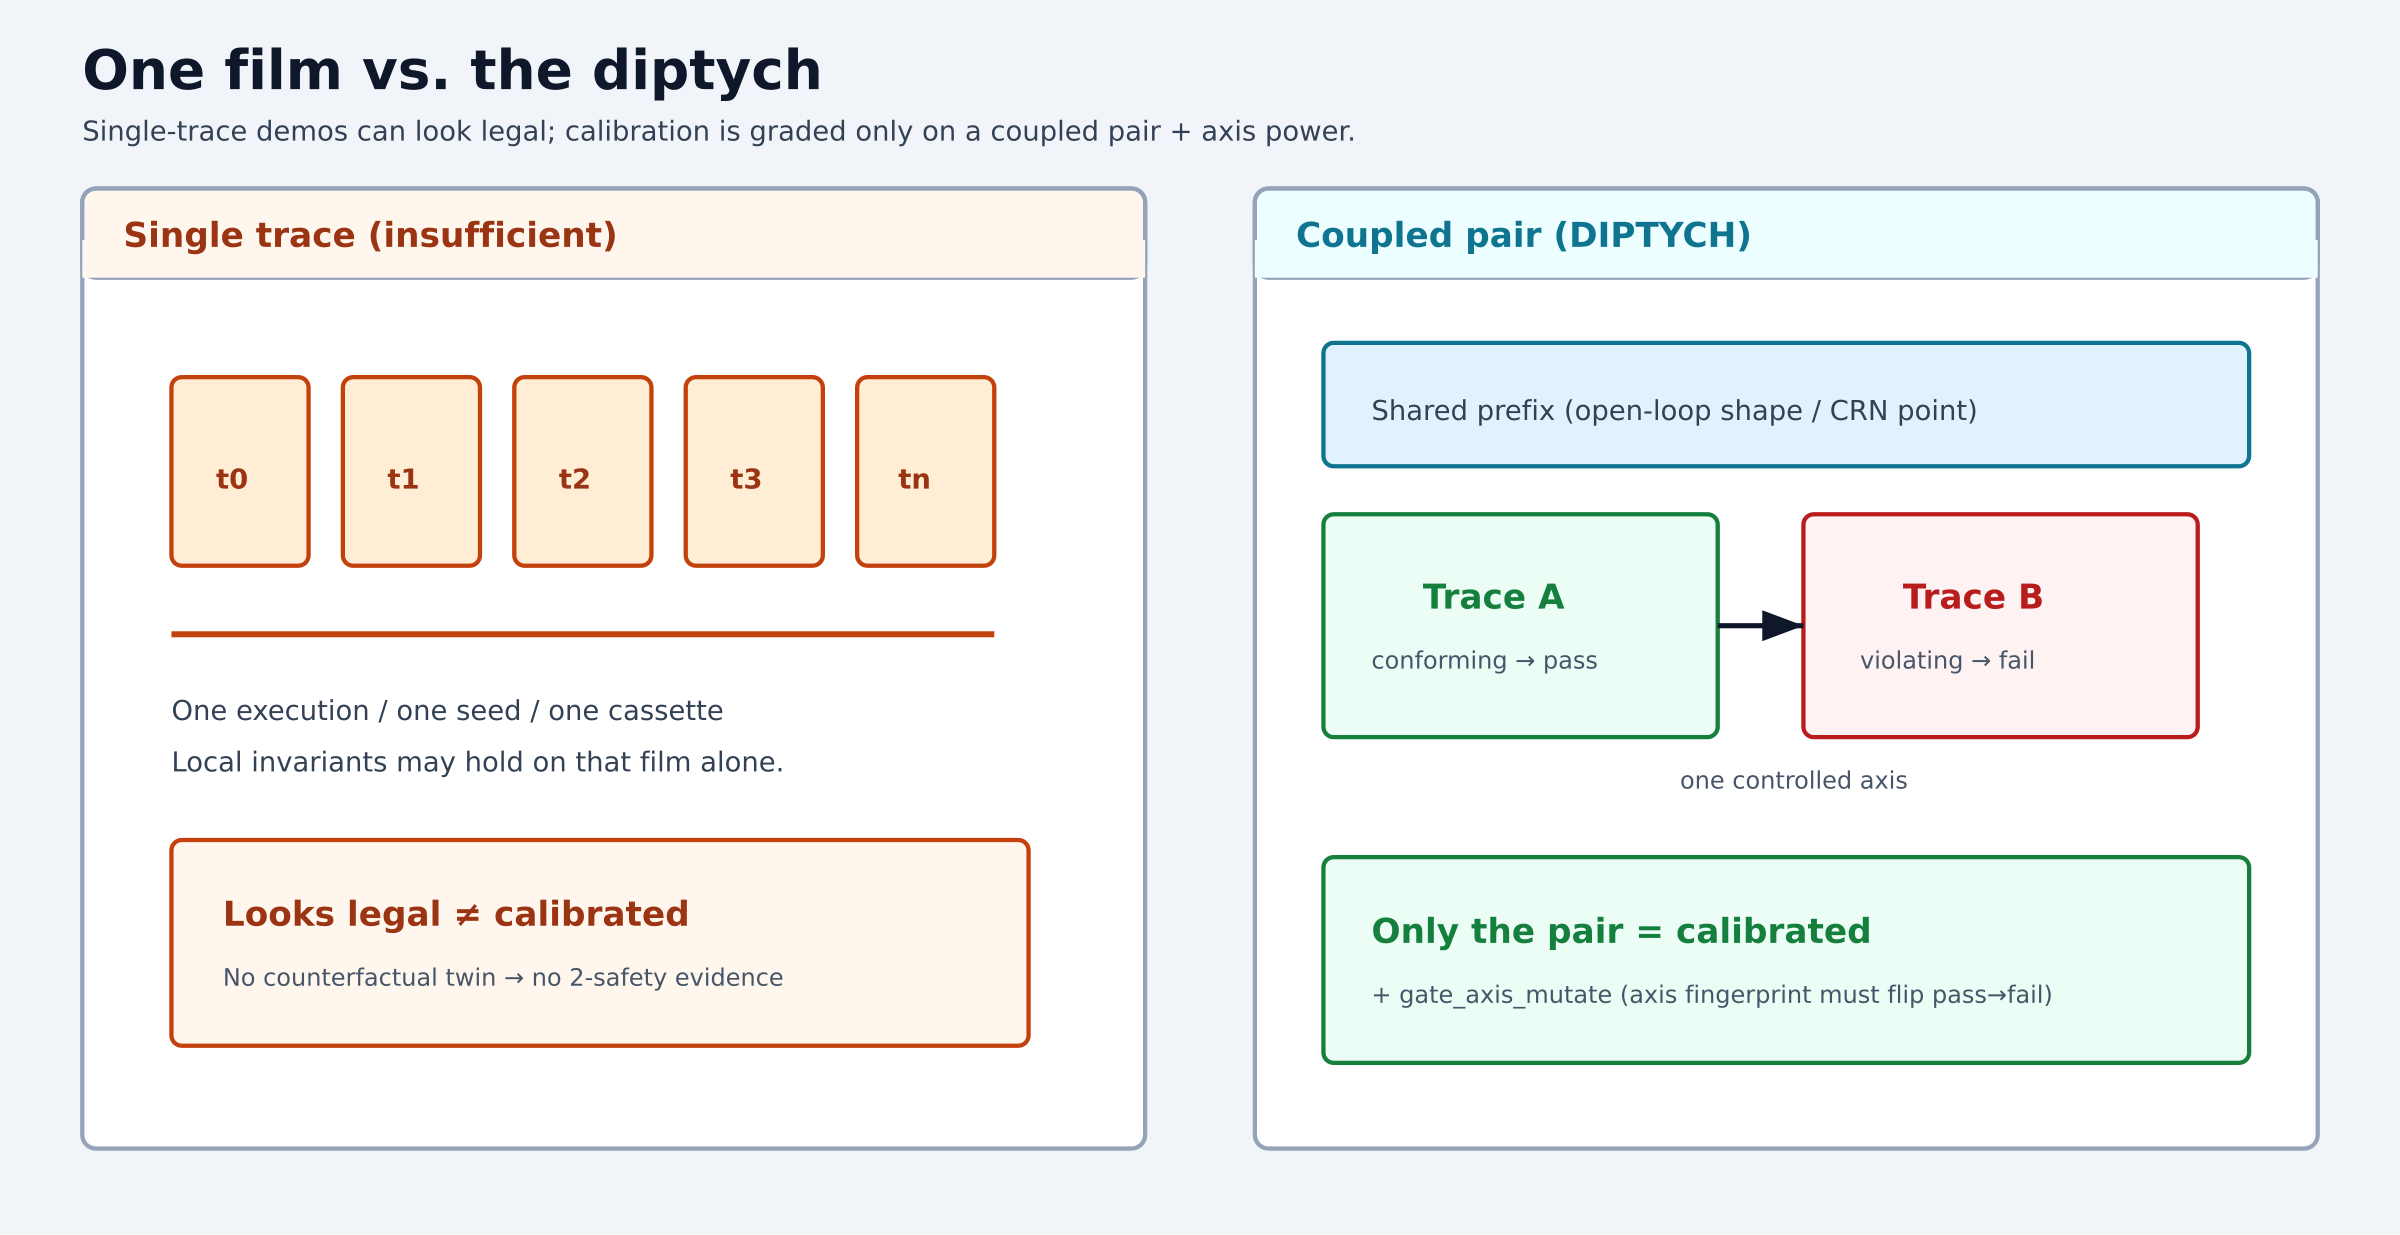
\includegraphics[width=0.8\columnwidth]{diptych-vs-single-trace.png}
		\caption{One film versus the diptych. Left: a single execution may satisfy
			local invariants yet provide no counterfactual twin. Right: calibration
			is graded only on a coupled pair that shares a prefix and differs on one
			controlled axis, with \texttt{gate\_axis\_mutate} requiring an axis-payload
			flip from pass to fail. Source: \texttt{docs/images/diptych-vs-single-trace.\{svg,png\}}.}
		\label{fig:diptych}
	\end{figure}
	
	\section{A Property Taxonomy for Agentic Evaluation}
	\label{sec:taxonomy}
	
	\subsection{Setup}
	
	We model an artifact as a deterministic transducer
	$A = (S, s_0, \delta, \lambda)$ over an observation alphabet $O$ and a
	decision alphabet $D$, with transition $\delta : S \times O \to S$ and
	output $\lambda : S \times O \to D$. Determinism is a requirement of the
	task, not an assumption of convenience; where an artifact is stochastic we
	take the seed to be part of the configuration.
	
	An execution on an observation sequence $\bar{o} = o_1 \ldots o_n$ yields a
	trace
	\[
	T = \exec(A, c, \bar{o}) = \langle (o_1, d_1), \ldots, (o_n, d_n) \rangle ,
	\]
	with $s_i = \delta(s_{i-1}, o_i)$ and $d_i = \lambda(s_{i-1}, o_i)$. Write
	$\Tr(A, c)$ for the set of traces $A$ produces over the workload family of
	interest.
	
	\begin{definition}[Trace property]
		A trace property is a set $P$ of traces. Artifact $A$ satisfies $P$ iff
		$\Tr(A,c) \subseteq P$.
	\end{definition}
	
	\begin{definition}[Hyperproperty]
		A hyperproperty is a set $H$ of \emph{sets} of traces. Artifact $A$
		satisfies $H$ iff $\Tr(A,c) \in H$ \cite{clarkson2010}.
	\end{definition}
	
	\begin{definition}[$k$-safety]
		A hyperproperty is $k$-safety if every violation is witnessed by a set of at
		most $k$ traces. A $k$-safety hyperproperty reduces to an ordinary safety
		property of the $k$-fold self-composition \cite{barthe2004,terauchi2005};
		testing it means executing the artifact $k$ times on related inputs and
		evaluating a predicate over the resulting tuple.
	\end{definition}
	
	The practical reading of $k$-safety is a cost statement. A $1$-safety
	requirement needs one run. A $2$-safety requirement needs a matched pair,
	and the matching is where the engineering lies.
	
	\subsection{The five classes}
	
	\textbf{Trace safety.} A bad prefix exists. One run falsifies. Example: a
	limit outside its configured bounds. These are cheap and are what current
	harnesses check well.
	
	\textbf{Quantitative trace properties.} A real-valued functional of one
	trace compared against a threshold. One long run falsifies, subject to
	sampling error. Example: mean latency error within a tolerance of the
	setpoint.
	
	\textbf{$k$-safety hyperproperties.} A tuple of $k$ traces falsifies; no
	single trace does. Almost everything in this paper is $k=2$. Example:
	asymmetric response, determinism, state round-trip stability.
	
	\textbf{Quantitative hyperproperties.} A comparator over a tuple of traces,
	with a threshold, rather than a boolean. Example: volatility suppression
	requires that the conservatism of the high-variance arm strictly dominate
	that of the low-variance arm, which is a real-valued contrast over a pair.
	
	\textbf{Resource properties.} Statements about execution cost rather than
	output. Example: median tick latency, or state size independent of tick
	count. These are single-trace but noisy,
	and require repetition for a different reason than $k$-safety does.
	
	Table \ref{tab:classes} summarizes the falsification evidence each class
	requires.
	
	\begin{table}[t]
		\caption{Evidence required to falsify, by property class}
		\label{tab:classes}
		\centering
		\small
		\begin{tabular}{@{}lll@{}}
			\toprule
			Class & Witness & Harness cost \\
			\midrule
			Trace safety & one bad prefix & one run \\
			Quantitative trace & one long run & one run \\
			$k$-safety hyper & matched $k$-tuple & $k$ coupled runs \\
			Quantitative hyper & contrast over tuple & $k$ coupled runs \\
			Resource & repeated timing & $r$ repetitions \\
			\bottomrule
		\end{tabular}
	\end{table}
	
	\section{Auditing a Public Specification}
	\label{sec:audit}
	
	How common are such requirements in specifications that practitioners
	actually write? We audited RFC~9743 \cite{rfc9743}, the IETF's 2025 Best
	Current Practice for specifying and assessing congestion control
	algorithms---adaptive rate controllers, the direct ancestors of
	concurrency limiters. Its Sections~5 and~7 state the criteria a proposed
	algorithm is evaluated against.
	
	\textbf{Method.} We took every criterion in those sections that
	constrains or asks for an evaluation of the algorithm's \emph{behavior}
	(18 in all), setting aside documentation duties (e.g., explaining
	deviations from earlier principles) and descriptions of environments. We
	classified each by one rule: a criterion needs \emph{paired} executions
	iff its text defines the quantity as an effect, impact, or harm relative
	to a reference situation, or as robustness to a change; otherwise it is
	a property of one run. Table~\ref{tab:audit} gives the result; the
	classification is ours and each row cites its section so it can be
	checked.
	
	\begin{table*}[t]
		\caption{The eighteen behavioral evaluation criteria of RFC~9743, paraphrased, with the evidence each requires. \emph{Paired} criteria are defined by a contrast between two executions.}
		\label{tab:audit}
		\centering
		\scriptsize
		\begin{tabular}{@{}llll@{}}
			\toprule
			RFC~9743 & Criterion (paraphrased) & Class & Contrast (if paired) \\
			\midrule
			\S5.1.1 & Full backoff or stop under persistent congestion & trace property & \\
			\S5.1.2 & Avoid maintaining excessive queues & quantitative trace & \\
			\S5.1.3 & Avoid causing high loss; reduce rate under high loss & quantitative trace & \\
			\S5.1.4 & How capacity is shared among flows of the same algorithm & quantitative trace & \\
			\S5.1.5 & How short-lived flows affect long-lived flows, and vice versa & \textbf{paired} & with vs.\ without the other flows \\
			\S5.2 & More harm than standard algorithms to flows sharing a bottleneck & \textbf{paired} & proposed vs.\ standard algorithm \\
			\S5.2 & No starvation; backoff when all feedback is lost & trace property & \\
			\S5.2.1 & Negative impact on flows using standard congestion control & \textbf{paired} & proposed vs.\ standard competitor \\
			\S5.2.2 & Coexistence with real-time congestion control & quantitative trace & \\
			\S5.2.3 & Effect on short and long flows using other algorithms & \textbf{paired} & with vs.\ without the proposed flows \\
			\S7.1 & Reaction to ECN congestion marks conforms to the codepoint & trace property & \\
			\S7.2 & Operates within the envelope of network circuit breakers & trace property & \\
			\S7.3 & Robust to a significant change in minimum delay & \textbf{paired} & with vs.\ without the delay change \\
			\S7.6 & Performance with misbehaving nodes or attackers & quantitative trace & \\
			\S7.8 & Performance under transient events & quantitative trace & \\
			\S7.9 & Impact of path changes; robust to them & \textbf{paired} & with vs.\ without the path change \\
			\S7.10 & Failover: harm to performance from a path change & \textbf{paired} & with vs.\ without failover \\
			\S7.10 & Concurrent multipath: harm to other flows at a shared bottleneck & \textbf{paired} & multipath vs.\ single-path flow \\
			\bottomrule
		\end{tabular}
	\end{table*}
	
	Three findings follow.
	
	\textbf{Eight of eighteen criteria are contrasts between executions.}
	They ask what an algorithm does \emph{to} something: to competing flows,
	relative to what a standard algorithm would have done to them, or to its
	own performance when the path changes. ``Harm'' in this sense is a
	two-run quantity by definition \cite{ware2019}: the same competitor is
	measured once against the proposed algorithm and once against the
	incumbent. The ten single-run criteria concern the algorithm's own
	absolute behavior---backoff, queue build-up, loss.
	
	\textbf{The contrasts are where the judgment is.} The paired criteria
	are the calibration questions: how aggressive toward others, how
	sensitive to change. A calibration requirement is a statement about how
	behavior would differ under a counterfactual input, and counterfactual
	contrasts are not single-trace objects. We expect this pattern to recur
	in any specification that asks for judgment rather than conformance.
	
	\textbf{The comparison is left unconstructed.} By its own account the
	document gives no thresholds, and it does not say what must be held
	fixed between the two runs---the path, the competing traffic, the random
	losses. Two evaluators can therefore reach different verdicts from the
	same algorithm, and the natural shortcut for the robustness criteria, a
	before/after comparison within one run, compares the algorithm at two
	different internal states. The next subsection shows why that shortcut
	fails, and Section~\ref{sec:harness} supplies the missing construction.
	
	\subsection{The obstruction}
	
	\begin{proposition}[State confounding]
		\label{prop:confound}
		Let $A$ be a deterministic transducer with decisions in a normed space
		$D$, and let $T = \exec(A, c, \bar{o})$ be a trace in which no state
		recurs ($s_i \neq s_j$ for $i \neq j$). For a visited state $s = s_{i-1}$
		with observation $o = o_i$ and a perturbation $e$ with
		$o \oplus e \neq o \neq o \ominus e$, define the sign contrast
		\[
		\rho_A(s, o, e) = \big\| \lambda(s, o \oplus e) - \lambda(s, o) \big\|
		- \big\| \lambda(s, o \ominus e) - \lambda(s, o) \big\| .
		\]
		Then there are transducers $A^{+}$ and $A^{-}$ with
		$\exec(A^{\pm}, c, \bar{o}) = T$ and
		$\rho_{A^{+}}(s,o,e) > 0 > \rho_{A^{-}}(s,o,e)$. Hence no function of $T$
		identifies $\rho$.
	\end{proposition}
	
	\begin{IEEEproof}
		$T$ constrains $\lambda$ only on the visited pairs $(s_{j-1}, o_j)$ and
		$\delta$ only along the path; by no recurrence, the only visited pair
		with state $s$ is $(s, o)$. Fix $u \in D$ with $u \neq 0$ and let $A^{+}$
		equal $A$ except $\lambda^{+}(s, o \oplus e) = \lambda(s,o) + 2u$ and
		$\lambda^{+}(s, o \ominus e) = \lambda(s,o) + u$; let $A^{-}$ swap the two
		values. Neither pair occurs in $T$ and $\delta$ is unchanged, so both
		transducers produce $T$, while $\rho_{A^{+}} = \|u\| > 0$ and
		$\rho_{A^{-}} = -\|u\| < 0$.
	\end{IEEEproof}
	
	This is the fundamental problem of causal inference \cite{holland1986}
	in transducer form: each state is observed under one input only. Any
	single-trace estimate of $\rho$ must borrow outputs from other states and
	so rests on an assumption relating $\lambda$ across states---exactly
	what calibration requirements leave open. Paired execution evaluates
	$\lambda(s, o \oplus e)$ and $\lambda(s, o \ominus e)$ directly by forking
	at $s$. The no-recurrence hypothesis is mild: a controller carrying
	real-valued estimators over a non-stationary stream essentially never
	revisits a state, and detecting recurrence would require the state
	inspection a black-box contract forbids.
	
	\section{\sys{}: Paired-Trace Grading}
	\label{sec:harness}
	
	\sys{} renders every hyperproperty judgment on two panels. Its design
	addresses three problems: constructing a valid pair, keeping the pair
	comparable in a closed loop, and paying for the extra executions.
	
	Execution and grading are separate. A \emph{probe} forks a running
	artifact at a shared state, drives two branches that differ on one axis,
	and only \emph{records} the pair into an \emph{envelope}: two traces of
	named value series plus the operator, coupling, and seed. A
	\emph{predicate} for the requirement then reads the envelope alone, after
	a comparability check common to all requirements. Hand-written control
	envelopes (with an expected verdict), envelopes emitted by external
	tools, and \emph{live} envelopes recorded from an artifact under test
	share this path, so every verdict can be recomputed offline from the
	saved envelope.
	
	\subsection{Coupling discipline}
	
	\begin{definition}[Exogenous coupling]
		Two executions are exogenously coupled if every input not causally derived
		from the artifact's own decisions is bit-identical between them, except for
		the single dimension the perturbation operator varies.
	\end{definition}
	
	Each probe declares one of two couplings. An \emph{open-loop} probe drives
	both arms with a fixed observation sequence after the shared prefix;
	decisions are graded but do not feed the plant, so coupling is exact and
	the probe isolates the response function of
	Proposition~\ref{prop:confound}. Six operators are open-loop. A
	\emph{CRN closed-loop} probe runs both arms against a live plant whose
	exogenous noise, arrivals, and faults come from a shared
	common-random-numbers stream \cite{glasserman1992}; the arms diverge only
	through the perturbation and the artifact's reaction. It measures
	outcomes---which operating point the system settles into---and is
	required for \textsc{TrajSwap} and \textsc{VarScale}; the envelope
	contract rejects open-loop tagging of either.
	
	\subsection{Comparability and inconclusive verdicts}
	
	\begin{definition}[Comparability]
		\label{def:horizon}
		A probe declares a horizon (length and unit). A twin pair is
		\emph{comparable} only while shared-prefix integrity holds over the
		horizon: both twins are present, paired channels have equal length,
		and CRN twins share a stream identifier.
	\end{definition}
	
	\begin{definition}[Inconclusive verdict]
		\label{def:inconclusive}
		A probe on a non-comparable pair returns \texttt{inconclusive}, with a
		recorded reason, instead of \texttt{pass} or \texttt{fail}. Inconclusive
		is never counted as a pass.
	\end{definition}
	
	Closed-loop residual bounds belong to the graded predicate, so exceeding
	them fails a probe; in the pilot, pairs whose branches hit a controller
	bound are inconclusive. Reporting inconclusive separately is deliberate:
	silently degrading a paired probe into a coin flip would reproduce, one
	level up, the failure this paper describes.
	
	\subsection{Probe trees and amortization}
	
	Naive $k$-safety grading multiplies cost by $k$. With deterministic replay,
	both arms share the prefix up to the perturbation point $t_p$, which need
	be executed only once. We count tick evaluations, not wall-clock time.
	
	\begin{proposition}[Prefix sharing]
		\label{prop:prefix}
		A $2$-safety probe with perturbation point $t_p$ and scenario length $n$
		costs $n + (n - t_p)$ tick evaluations under exogenous coupling, rather
		than $2n$.
	\end{proposition}
	
	\begin{corollary}[Probe tree]
		\label{cor:tree}
		$m$ probes sharing $t_p$ cost $C_{\mathrm{tree}} = t_p + \sum_{j}(n_j -
		t_p)$ rather than $C_{\mathrm{naive}} = \sum_j 2 n_j$; the marginal cost
		of a late-forking probe approaches its suffix length.
	\end{corollary}
	
	\begin{definition}[Amortization factor]
		\label{def:cost}
		$\alpha = C_{\mathrm{naive}} / C_{\mathrm{tree}}$;
		Section~\ref{sec:eval-cost} reports it on live executions.
	\end{definition}
	
	Forking needs a cheap copy of artifact state at $t_p$. Our task already
	mandates snapshot/restore with bit-identical continuation
	(\textsc{FreezeDry}'s axis), so the property that makes an artifact
	restartable also makes paired grading affordable; we suggest task
	specifications require it for that reason alone.
	
	\subsection{Power-on-axis: \texttt{gate\_axis\_mutate}}
	
	Twin contrast alone is not enough: identical twins with hard-coded
	opposite expected verdicts look green. \sys{} therefore mutates
	\emph{only} the operator's graded axis of each conforming twin (seed,
	freeze mask, schema key, polarity, saturation bound, history splice,
	trajectory segment, or variance scale), demands a \texttt{pass}$\to$%
	\texttt{fail} flip with a recorded before/after witness, and requires
	that a wrong-axis mutation \emph{not} flip. A coverage cell is green only
	when conforming passes, violating fails, and the gate reports power.
	
	\section{Perturbation Operators}
	\label{sec:operators}
	
	An operator takes a scenario and returns a twin, varying one semantic
	dimension and preserving everything else. Table \ref{tab:ops} lists the
	eight operators in \sys{}.
	
	\begin{table}[t]
		\caption{Perturbation operators: coupling (OL open-loop, CRN
			closed-loop), the varied axis, and the requirement probed.}
		\label{tab:ops}
		\centering
		\scriptsize
		\begin{tabular}{@{}llll@{}}
			\toprule
			Operator & Coup. & Varies & Probes \\
			\midrule
			\textsc{SignFlip}  & OL  & sign of deviation & asymmetric response \\
			\textsc{TrajSwap}  & CRN & order of recent samples & trend recency \\
			\textsc{VarScale}  & CRN & noise variance & volatility suppression \\
			\textsc{SatExtend} & OL  & saturation duration & anti-windup \\
			\textsc{HistSwap}  & OL  & pre-step history & setpoint-change quiet \\
			\textsc{FreezeDry} & OL  & serialize/restore & round-trip stability \\
			\textsc{Reseed}    & OL  & process / hash seed & determinism \\
			\textsc{SchemaX}   & OL  & scenario & schema stability \\
			\bottomrule
		\end{tabular}
	\end{table}
	
	Three constructions deserve a note.
	\textsc{TrajSwap} permutes samples inside a window (multiset-fixed) so one arm
	ends improving and the other degrading; order-insensitive summaries fail by
	construction (the pilot scripts this window open-loop; the closed-loop
	form is the one external tools emit). \textsc{SatExtend} pairs a saturated arm with its
	extension and requires every actuator sample on both arms to stay inside
	the declared saturation and legal bounds, which an unbounded integrator
	exceeds; the recorded-envelope grader checks
	these bounds, while the pilot's live probe (Section~\ref{sec:pilot})
	compares the first post-release response directly.
	\textsc{SchemaX} compares emission records across scenarios ($2$-safety
	over a trace set rather than a perturbation pair), catching drift no
	single scenario exhibits; drift within one run is single-trace
	falsifiable, which our strong baseline exploits.
	
	\section{Metrics}
	\label{sec:metrics}
	
	\subsection{Probe power}
	
	For each operator, power against Section~\ref{sec:protocol} controls is the
	fraction of violating controls on which the probe returns fail and conforming
	controls on which it returns pass. A probe that cannot separate its own
	control pair is not used.
	
	\subsection{Separation index}
	
	For artifacts $A,B$, let $\mathrm{eq}_{\mathrm{tr}}(A,B)$ hold when their
	trace-property score vectors agree within tolerance. The separation index is
	the fraction of such pairs on which hyperproperty score vectors disagree.
	Near zero refutes the premise; near one shows paired probes carry information
	trace grading cannot recover.
	
	\subsection{Cost}
	
	Proposition~\ref{prop:prefix}, Corollary~\ref{cor:tree}, and
	Definition~\ref{def:cost} give the cost model. We count tick evaluations,
	not wall-clock time or dollars.

	\subsection{Grader adequacy}
	\label{sec:adequacy-metric}

	For a conforming probe and a single-leaf mutation of its traces, call the
	mutant \emph{on-axis} if it changes the operator's declared graded-axis
	snapshot and \emph{off-axis} otherwise. The \emph{on-axis kill rate} is the
	fraction of on-axis mutants the grader does not pass; the \emph{off-axis
	fail rate} is the fraction of off-axis mutants graded \texttt{fail}, which
	measures dependence on fields outside the declared axis.
	
	\section{Evaluating the Harness}
	\label{sec:protocol}
	
	We ask two questions. Do \sys{}'s graders reject what they claim to reject
	(ground-truth controls, a power-on-axis gate, an exhaustive mutation
	sweep)? And does paired grading change the verdict on controllers that
	models actually write (a pilot study)? Every number below is produced by a
	command in the public artifact (Artifact availability,
	Section~\ref{sec:conclusion}).
	
	\subsection{Ground-truth controls}
	
	For each operator we hand-author three recorded probe pairs whose verdict
	is known by construction: \emph{conforming}, \emph{violating} (one design
	decision changed on the graded axis), and \emph{incomparable} (must be
	\texttt{inconclusive}). All 24 grade as expected. These are controls, not
	findings. A five-envelope \emph{cosmetic} corpus (injected AUROC field,
	hard-coded pass, missing axis, stub marker, wrong schema version) is
	rejected 5/5.
	
	\subsection{Power-on-axis and adapter coverage}
	\label{sec:adapters}
	
	For all 24 operator--source cells of the coverage matrix
	(\texttt{coverage/matrix.json}), the conforming twin passes, the violating
	twin fails, and \texttt{gate\_axis\_mutate} flips pass$\to$fail when only the named axis
	is mutated while a wrong-axis distractor does not flip. Besides our core
	fixtures, the sources are two external tools that emit
	schema-\texttt{0.2} twins from their own executions, testing that the
	envelope contract works outside the harness: ZeroDay, a
	vulnerability-localization tool whose probes perturb its ranking and
	search (e.g., the sign of a score margin), and AOMB, an agent that tunes a
	small language model for telemetry anomaly detection. Both are the
	authors' own open-source projects, pinned at commits \texttt{fb5b39da}
	and \texttt{667e475}. A green cell means grader and emitter agree on the
	axis, not that either tool is correct.
	
	
	
	\subsection{Grader adequacy: an exhaustive mutation sweep}
	\label{sec:eval-adequacy}
	
	The coverage matrix says each grader separates \emph{one} hand-picked
	mutation. It does not say the grader is sensitive to its whole axis. We
	therefore mutate every scalar leaf under \texttt{traces} of all 18
	conforming probes (core cassette, core probes, and adapter fixtures) with
	every applicable single-leaf edit (negate and shift numbers, toggle
	booleans, suffix strings, fill nulls), yielding 1{,}030 mutants: 827
	on-axis and 203 off-axis (Section~\ref{sec:adequacy-metric}). A surviving
	on-axis mutant is either a legitimate insensitivity of the predicate or a
	grader blind spot; we triage every one.
	
	\textbf{Defects found.} The first sweep killed 557 of 827 on-axis mutants
	(67.4\%) and surfaced three classes of defect in our own graders.
	\emph{Self-reported evidence bypass:} \textsc{SignFlip} passed whenever
	the twins carried equal emitter-supplied fingerprints, short-circuiting
	the check on the data (90 of 93 on-axis mutants survived).
	\emph{One-sided bound:} \textsc{TrajSwap} checked residuals as $r \le b$
	rather than $|r| \le b$. \emph{Twin-asymmetric parameters:} four graders
	read bounds and tolerances from the first twin only, so the second could
	declare anything. After the fixes the kill rate is 82.5\%
	(\textsc{SignFlip} 3.2\%$\to$93.5\%, \textsc{SatExtend}
	30.6\%$\to$51.0\%, \textsc{Reseed} 85.7\%$\to$93.8\%, \textsc{VarScale}
	92.5\%$\to$100\%); no verdict on any shipped control, adapter fixture, or
	coverage cell changed, and each defect is pinned by a regression test.
	
	\textbf{Survivors.} Of the 145 surviving on-axis mutants, 133 are
	legitimate insensitivities (e.g., edits that stay inside a declared
	bound) and 12 are blind spots: two fields declared on-axis but never
	read. All 99 off-axis mutants graded \texttt{fail} hit preconditions the
	axis declaration omits; axis declarations should be derived from the
	grader, not written beside it.
	
	\subsection{Pilot: model-authored controllers on two tasks}
	\label{sec:pilot}
	
	\textbf{Tasks.} Task~A is the concurrency controller of
	Section~\ref{sec:motivating}; we wrote its eight requirements, one per
	operator. Task~B is a congestion control algorithm for a simulated
	drop-tail bottleneck. Its eight requirements paraphrase RFC~9743
	criteria (Table~\ref{tab:audit}): three single-run (full backoff, rate
	reduction under loss, fairness within the algorithm) and five paired
	(throughput and latency harm to a standard Reno flow relative to a
	Reno competitor, harm to short flows, robustness to a delay change and
	to a path change). The RFC gives no thresholds, so those are ours, as
	are two performance goals the standard algorithm does not meet (useful
	throughput under random loss; a short queue), which give a reason to
	depart from it. Task~B needed two perturbations beyond the eight
	operators---substituting a reference algorithm for the candidate, and
	stepping a path parameter on one arm---and the envelope pipeline took
	both unchanged. Both simulators pre-draw their noise from a seed, so
	paired runs share it. Probes run at several fork points and three
	seeds; a violation at any of them fails the requirement.
	
	\textbf{Single-trace baselines.} The \emph{basic} baseline implements,
	per requirement, the check a harness author would write from its prose
	on one run---for asymmetric response, the ratio of mean downward to
	upward limit moves; for harm, the standard flow's share of the link.
	The \emph{strong} baseline gives single-trace grading every advantage
	we could find: two or three readings per requirement (regression
	slopes, trend coefficients, Jain's index, queue percentiles) over every
	applicable scenario, failing if any reading fires. Like the paired
	probes, no reading may flag the conforming control.
	
	\textbf{Executable controls.} Each task has a conforming controller and
	eight violators that change one design decision. Paired grading catches
	all sixteen violators on their own requirement. The basic and strong
	baselines catch one and three of eight on Task~A, and seven and eight of
	eight on Task~B. Building the controls was instructive: two first-draft
	Task~A violators \emph{satisfied} the requirements they were meant to
	break, because requirements interact (asymmetric gain already
	suppresses volatility). A violator is only a violator once a probe says
	so.
	
	\textbf{Artifacts.} Eighty controllers, forty per task, from four
	conditions: five one-shot, tool-free samples from each of four Claude
	models (Haiku~4.5, Sonnet~5, Opus~5.5, Fable~5.1); five one-shot samples
	from OpenAI's \texttt{gpt-5.6-sol} via Codex; and ten Claude and five
	Codex samples in an \emph{agentic} condition, where the agent works in a
	directory with the task, the simulator (for Task~B, including the
	standard algorithm to compete against), and its own tests, but never
	sees our probes. All 80 load and run; forking by state copy matched
	replay-from-scratch for every one.
	
	\begin{table}[t]
		\caption{Pilot on 80 model-written controllers. \emph{single}:
			pass every basic single-trace check; \emph{viol.}: of those, fail a
			paired probe; \emph{clean}: pass every requirement under full
			grading.}
		\label{tab:pilot}
		\centering
		\scriptsize
		\begin{tabular}{@{}lrrrrrrr@{}}
			\toprule
			& & \multicolumn{3}{c}{Task A (ours)} & \multicolumn{3}{c}{Task B (RFC 9743)} \\
			Condition & $n$ & single & viol. & clean & single & viol. & clean \\
			\midrule
			One-shot, Claude & 20 & 15 & 12 & 2 &  6 & 2 & 4 \\
			One-shot, Codex  &  5 &  4 &  3 & 1 &  0 & 0 & 0 \\
			Agentic, Claude  & 10 & 10 &  8 & 2 &  6 & 0 & 6 \\
			Agentic, Codex   &  5 &  5 &  5 & 0 &  4 & 1 & 3 \\
			\midrule
			All              & 40 & 34 & 28 & 5 & 16 & 3 & 13 \\
			\bottomrule
		\end{tabular}
	\end{table}
	
	\textbf{Task A: a single trace misses most violations.} 34 of 40
	controllers pass every basic single-trace check, and 28 of those violate
	a stated requirement under paired probing (82\%, 95\% Wilson CI
	66--92\%; per controller, 33 paired-only vs.\ 2 single-only detections,
	exact McNemar $p<10^{-7}$). Trend recency dominates (23 violations, one
	caught): most controllers add a trend term too weak to overcome their
	estimator lag, so after improving latency the limit ends \emph{lower}
	than after the same observations worsening. Volatility suppression
	fails for 13, asymmetric response for 10, anti-windup and
	setpoint-change quiet for 3 each. Because several Task~A requirements
	are stated comparatively, a single-trace check can only approximate
	them; the result is how often controllers violate requirements given
	to them in plain words, not that an approximation errs.
	
	\textbf{Task B: a single trace is often enough.} 27 of 40 controllers
	violate at least one requirement, but here the basic baseline finds
	most of it: of the 16 controllers it passes, 3 fail a paired probe
	(19\%, CI 7--43\%). Harm to a standard flow, the RFC's central
	comparative criterion, was caught in a single run in all 15 cases. The
	ten violations only pairing found (nine controllers; McNemar $p=0.004$)
	are path change (5 of 5 missed), short flows (3 of 7), and delay change
	(2 of 14). One agentic controller loses 97\% of its throughput when the
	delay doubles at tick 350 but not at tick 250, which a single run with
	one change point cannot see; another keeps a standing queue four times
	larger after a capacity drop than on a path that was always slow.
	
	\textbf{When is one trace enough?} The two tasks differ in where the
	reference arm of the contrast comes from. For harm, the reference
	outcome is a constant the harness knows in advance---a standard flow's
	fair share is half the link---so one run against that constant
	suffices. For Task~A's requirements and Task~B's path, delay, and
	short-flow requirements, the reference is the same artifact from the
	same state under a different input, or with a different history; no
	constant stands in for it, and that is where single-trace grading
	failed. This is Proposition~\ref{prop:confound} read as a design rule:
	pair when the reference depends on the artifact's own state.
	
	\textbf{Stronger baselines err differently.} On Task~A the strong
	baseline flags 29 controllers, yet 10 of the 11 it passes violate a
	requirement, and on asymmetric response it disagrees with the
	fixed-state contrast on 25 of 40 (4 missed, 21 flagged that satisfy the
	requirement at all three seeds). On Task~B its Jain's-index reading
	flags 29 controllers for throughput harm that cause none: they take
	\emph{less} than their share, the known objection to fairness as a
	proxy for harm \cite{ware2019}.
	
	\textbf{Agents fix what they can observe.} On Task~A every agentic
	controller passes every basic single-trace check, yet 13 of 15 violate
	a requirement, three with integrator windup: the simulator shows one
	run, and agents polished one run. On Task~B the simulator shows the
	candidate beside a standard flow, and 9 of 15 agentic controllers are
	clean against 4 of 25 one-shot. With five samples per cell we make no
	model or vendor comparison.
	
	\textbf{Stability and cost.}
	\label{sec:eval-cost}
	3.1\% of Task~A paired verdicts are inconclusive (a branch hit a bound
	or never saturated); none on Task~B. Forked verdicts agree across seeds
	in 88\% (A) and 93\% (B) of cases, and 26 of the 55 paired-only
	violations hold at all three seeds; the any-seed rule resolves the rest
	conservatively. Counting executed controller ticks, prefix sharing
	gives $\alpha = 3.09$ on Task~A (254{,}076 vs.\ 784{,}476) and
	$1.45$ on Task~B (546{,}000 vs.\ 792{,}000), where reference-swap probes
	share no candidate prefix (Definition~\ref{def:cost}).
	\label{sec:future}
	
	\section{Related Work}
	\label{sec:related}
	
	\textbf{Hyperproperties / relational verification.} Clarkson and Schneider
	\cite{clarkson2010} with HyperLTL/HyperCTL$^*$ \cite{clarkson2014},
	model checking \cite{finkbeiner2015}, information-flow
	\cite{dimitrova2014}, observational determinism
	\cite{roscoe1995,zdancewic2003}, and self composition
	\cite{barthe2004,terauchi2005}. We do not extend that theory; we observe
	that agentic benchmarks depend on it unrecognized, and ship a pair harness.
	Differential privacy \cite{dwork2006,dwork2014} is likewise relational; we
	target calibration, not $(\varepsilon,\delta)$ budgets.
	
	\textbf{Testing and monitoring $k$-safety.} Runtime verification of
	HyperLTL monitors $k$-safety over sets of recorded traces
	\cite{agrawal2016,finkbeiner2019}, building on single-trace RV
	\cite{leucker2009,bartocci2018,falcone2018}; relational program logics
	verify $k$-safety statically \cite{sousa2016}. Closest to us, Christakis
	et al.\ specify and test $k$-safety properties of machine-learning
	models by generating related inputs \cite{christakis2023}. Those models
	are stateless; our artifacts are stateful closed-loop controllers, where
	the pair must share a prefix and a noise stream \cite{glasserman1992},
	and where Proposition~\ref{prop:confound} makes recorded traces
	insufficient---monitors over logged executions cannot supply the
	unvisited branch.
	
	\textbf{Metamorphic and property-based testing.} Metamorphic relations
	are $k$-safety under another vocabulary \cite{chen1998,segura2016},
	applied to autonomous systems by perturbing inputs \cite{tian2018};
	property-based testing checks universally quantified properties on
	random inputs \cite{claessen2000}. We add forking from a shared internal
	state, closed-loop coupling, and an explicit inconclusive verdict, and we
	test the graders themselves with mutation analysis \cite{jia2011}.
	
	\textbf{Evaluating model-written code.} Repository, tool-use, and
	functional-correctness benchmarks
	\cite{jimenez2024,yao2024,liu2023,zhou2024,chen2021} grade single
	executions or aggregates; EvalPlus showed that stronger tests overturn
	many pass verdicts \cite{liu2023evalplus}. Our pilot finds the same
	effect along a different axis: not more inputs, but paired executions.
	
	\textbf{Differential testing} compares implementations on shared inputs
	\cite{mckeeman1998}; we compare one implementation on deliberately
	related inputs.
	
	\section{Discussion}
	\label{sec:discussion}
	
	\textbf{A green matrix is necessary, not sufficient.} Every cell of
	the coverage matrix was green \emph{before} the mutation sweep, while
	\textsc{SignFlip} was passing 97\% of its on-axis mutants. One hand-picked
	mutation per axis certifies that a grader \emph{can} fail, not that it
	fails on the whole axis. We think any paired-grading harness, including
	ours, should report an exhaustive or sampled mutation sweep alongside its
	coverage matrix; self-reported evidence (fingerprints, hashes, summary
	flags) should never short-circuit a check on the underlying data.
	
	\textbf{Pair when the reference depends on the artifact.} The pilot does
	not show that single-trace grading always fails. It shows a boundary: a
	threshold in one run works when the other arm of the contrast is a
	constant known to the harness, and fails when the other arm is the
	artifact itself from the same state or with a different history. A
	benchmark author can apply this to each requirement before writing a
	check.
	
	\textbf{Non-claims.} A green cell is not a vulnerability finding, and no
	result here is an accuracy, AUROC, or model ranking; the envelope
	contract rejects such fields.
	
	\section{Threats to Validity}
	\label{sec:threats}
	
	\textbf{Audit.} The classification of RFC~9743 is ours, of one document
	that guides human evaluation rather than specifying a benchmark; moving
	the borderline rows (\S5.2.2, \S7.6, \S7.8) gives 8 to 11 paired
	criteria of 18.
	\textbf{Construct.} Operators encode one reading of each requirement; we
	publish them as code so intent disputes become artifact disputes.
	
	\textbf{Adapter pin drift.} Adapter greens hold at the pinned SHAs only;
	a pin move can flip them while core cells stay green.
	
	\textbf{Inconclusive.} Overusing it could hide weak probes; the pilot's
	3.1\% rate comes from branches hitting limit bounds or never saturating.
	
	\textbf{Handwritten-control bias.} Controls and fixtures are written by the
	same authors as the graders and can overfit them; the mutation sweep is
	our main mitigation, and it did find defects the controls had hidden. The
	sweep is itself bounded: it applies single-leaf edits only, so it cannot
	reveal defects that need coordinated multi-field changes, and its axis
	classification relies on the same declared snapshots whose
	incompleteness it exposed (Section~\ref{sec:eval-adequacy}).
	
	\textbf{Open-loop vs.\ CRN.} Open-loop greens do not transfer to the
	two closed-loop operators, and CRN coupling is not universal; on Task~A
	seed instability concentrates in closed-loop \textsc{VarScale}.
	
	\textbf{Pilot validity.} We wrote Task~A's requirements, Task~B's
	thresholds and performance goals, both simulators, and both baselines,
	calibrated on our own controls; a different single-trace design could
	catch more, though Proposition~\ref{prop:confound} bounds what any can
	identify. Paired verdicts are ground truth only relative to our reading
	of each requirement, and Task~B's fluid simulator is far simpler than a
	real network. Artifacts are 80 samples from two vendors, five per model,
	condition, and task; 7--12\% of forked verdicts depend on the noise
	seed.

	\textbf{External.} Findings come from one task family: we claim
	generality for the classification and harness architecture, not the
	operator set. Grading is deterministic, so every number in
	Section~\ref{sec:protocol} is exactly reproducible.
	
	\section{Conclusion}
	\label{sec:conclusion}
	
	Agentic benchmarks grade one trace at a time, yet many requirements on
	agent-authored systems---especially calibration---are only falsifiable as
	$2$-safety hyperproperties. We audited the IETF's evaluation criteria for
	congestion controllers (eight of eighteen behavioral criteria are
	contrasts between executions), proved the single-trace
	confound for stateful artifacts, and presented a paired harness with
	coupling, an inconclusive verdict, and a probe-tree cost model. A mutation
	sweep on our own graders found three classes of defect that a fully green
	coverage matrix had hidden. A pilot on 80 model-written controllers
	located the boundary: where a requirement compares an artifact with
	itself from the same state, most controllers that pass every
	single-trace check violate it; where the reference is a constant the
	harness already knows, one run suffices. When the counterfactual depends
	on the artifact, it needs two executions---and the grader that compares
	them needs testing too.
	
	{\raggedright\textbf{Artifact availability.}
	\url{https://github.com/pandeyaby/DIPTYCH} (MIT): code, controls, and all 80
	controllers. Section~\ref{sec:eval-adequacy}: \texttt{python -m
	diptych.adequacy}; Table~\ref{tab:pilot}: \texttt{python -m
	diptych.pilot.study [--task congestion]}.\par}
	
	\balance
	
	\bibliographystyle{IEEEtran}
	\bibliography{refs}
	
\end{document}
